	% Unit II.
	\chapter*{Unit II}
	\setcounter{questionnumber}{0}

	% 1.
	\begin{qanda}
		\begin{question}
How does looking at something underwater affect its apparent size?
		\end{question}

		\begin{answer}
Things look larger and/or closer.
		\end{answer}
	\end{qanda}

	% 2.
	\begin{qanda}
		\begin{question}
How does water affect light intensity and color?
		\end{question}

		\begin{answer}
Water absorbs and reflects light, so in deeper water it is darker and less colorful.
		\end{answer}
	\end{qanda}

	% 3.
	\begin{qanda}
		\begin{question}
How does being underwater affect hearing?
		\end{question}

		\begin{answer}
Sound travels farther in water than in air, so you'll be able to hear things at distances that you can't in air.  Sound also travels about four times faster in water than in air, this makes it difficult to tell where a sound comes from.
		\end{answer}
	\end{qanda}

	% 4.
	\begin{qanda}
		\begin{question}
How does the rate of body heat loss in water compare to the rate of body heat loss in air?
		\end{question}

		\begin{answer}
Water conducts heat 20 times faster than air.
		\end{answer}
	\end{qanda}

	% 5.
	\begin{qanda}
		\begin{question}
What should you do if you begin to shiver continuously underwater?
		\end{question}

		\begin{answer}
Get out of the water immediately, dry off, and seek warmth.
		\end{answer}
	\end{qanda}

	% 6.
	\begin{qanda}
		\begin{question}
How should you move underwater to compensate for the increased resistance of water?
		\end{question}

		\begin{answer}
Conserve energy by moving slowly and steadily.  Swim level to reduce drag.  More weight means you have to use more air in your BCD, which prevents you from swimming horizontally.
		\end{answer}
	\end{qanda}

	% 7.
	\begin{qanda}
		\begin{question}
How do you breathe underwater for maximum efficiency?
		\end{question}

		\begin{answer}
Slowly and deeply.
		\end{answer}
	\end{qanda}

	% 8.
	\begin{qanda}
		\begin{question}
What are eight symptoms of diving overexertion?
		\end{question}

		\begin{answer}
Overexertion symptoms include fatigue, labored breathing, a feeling of suffocation, weakness, anxiety, headache, muscle cramping and a tendency to panic.
		\end{answer}
	\end{qanda}

	% 9.
	\begin{qanda}
		\begin{question}
How do you prevent diving overexertion?
		\end{question}

		\begin{answer}
You prevent overexertion by staying relaxed and knowing your limits.
		\end{answer}
	\end{qanda}

	% 10.
	\begin{qanda}
		\begin{question}
What should you do if you become overexerted while diving -- either at the surface or underwater?
		\end{question}

		\begin{answer}
Stop all activity and rest underwater.  At surface, establish buoyancy and stop moving.  One you recover, continue at a slower pace.
		\end{answer}
	\end{qanda}

	% 11.
	\begin{qanda}
		\begin{question}
What are four techniques used for airway control?
		\end{question}

		\begin{answer}
Proper airway control means to:
			\begin{nospacenumberedlist}
				\item Always inhale slowly if water enters your regulator, snorkel or mouth, so you don't pull it into your throat
				\item Always inhale cautiously and slowly after clearing your snorkel or regulator
				\item Use your tongue as a splash guard by putting the tip on the roof of your mouth when you breath past small amounts of water
				\item Looking downward slightly helps keep the water in the second stage and out of your mouth
			\end{nospacenumberedlist}
		\end{answer}
	\end{qanda}

	% 12.
	\begin{qanda}
		\begin{question}
What are the two reasons for wearing an exposure suit while diving?
		\end{question}

		\begin{answer}
To reduce heat loss and to protect you from minor scrapes, stings and abrasions.
		\end{answer}
	\end{qanda}

	% 13.
	\begin{qanda}
		\begin{question}
How do dry suits and wet suits insulate divers?
		\end{question}

		\begin{answer}
By putting a layer of insulation over your skin.
		\end{answer}
	\end{qanda}

	% 14.
	\begin{qanda}
		\begin{question}
Why must a wet suit fit snugly?
		\end{question}

		\begin{answer}
To prevent water from circulating through it.  If water circulates you lose heat to incoming cold water.
		\end{answer}
	\end{qanda}

	% 15.
	\begin{qanda}
		\begin{question}
What two properties may an exposure suit lose due to increased water pressure at depth?
		\end{question}

		\begin{answer}
Buoyancy and insulation.
		\end{answer}
	\end{qanda}

	% 16.
	\begin{qanda}
		\begin{question}
What three factors should you consider when selecting an exposure suit?
		\end{question}

		\begin{answer}
Insulating ability, fit, and comfort.
		\end{answer}
	\end{qanda}

	% 17.
	\begin{qanda}
		\begin{question}
What four procedures apply to caring for an exposure suit?
		\end{question}

		\begin{answer}
Exposure suits have four basic maintenance steps:
			\begin{nospacenumberedlist}
				\item Rinse
				\item Dry inside out
				\item Store
				\item Lubricate dry suit zippers periodically
			\end{nospacenumberedlist}
		\end{answer}
	\end{qanda}

	% 18.
	\begin{qanda}
		\begin{question}
Why do you need a hood and what are the three basic types of hoods?
		\end{question}

		\begin{answer}
You loose body heat through your head.  75 percent if wearing a full body exposure suit, but leave your head uncovered.  The three basic types are bibbed hoods, non-bibbed hoods, and hooded vests.
		\end{answer}
	\end{qanda}

	% 19.
	\begin{qanda}
		\begin{question}
Why should you avoid an excessively tight-fitting hood?
		\end{question}

		\begin{answer}
A hood that is too tight can compress arteries in your neck, which the brain perceives as high blood pressure and then lowers your heart rate.
		\end{answer}
	\end{qanda}

	% 20.
	\begin{qanda}
		\begin{question}
What are two reasons for wearing dive gloves?
		\end{question}

		\begin{answer}
To protect against heat loss and injuries.
		\end{answer}
	\end{qanda}

	% 21.
	\begin{qanda}
		\begin{question}
What are three reasons for wearing wet suit boots while diving?
		\end{question}

		\begin{answer}
Warmth, protection against injuries while walking to and from the water, and for comfort when wearing adjustable-strap fins.
		\end{answer}
	\end{qanda}

	% 22.
	\begin{qanda}
		\begin{question}
In what six ways can you prevent overheating before a dive when wearing an exposure suit?
		\end{question}

		\begin{answer}
The six ways to prevent overheating are:
			\begin{nospacenumberedlist}
				\item Set up all your equipment before putting on the exposure suit and then put the suit on at the last possible moment
				\item Once you have the suit on, limit your activity as much as possible
				\item Stay out of the sun as much as possible
				\item keep your hood off, of at least pulled back off your head as long as possible
				\item Leave your jacket unzipped as long as possible
				\item Cool off by entering the water, or spraying down with a hose
			\end{nospacenumberedlist}
		\end{answer}
	\end{qanda}

	% 23.
	\begin{qanda}
		\begin{question}
What are two types of weight systems?
		\end{question}

		\begin{answer}
The wight belt and the integrated weight system.
		\end{answer}
	\end{qanda}

	% 24.
	\begin{qanda}
		\begin{question}
What's the most important feature of any weight system?
		\end{question}

		\begin{answer}
The quick release feature.
		\end{answer}
	\end{qanda}

	% 25.
	\begin{qanda}
		\begin{question}
How do you determine how much weight you need for a dive?
		\end{question}

		\begin{answer}
With your regulator in, your BCD deflated, and holding a normal breath you should have enough weight to float at eye level.  When you exhale you should slowly descend.  Then add 5 pounds to offset the air you will loose from your cylinder.
		\end{answer}
	\end{qanda}

	% 26.
	\begin{qanda}
		\begin{question}
What's an alternate air source?
		\end{question}

		\begin{answer}
Any second stage you may use, other than your own primary second stage, to ascend while breathing normally.
		\end{answer}
	\end{qanda}

	% 27.
	\begin{qanda}
		\begin{question}
What two types of alternate air source require the help and cooperation of another diver?
		\end{question}

		\begin{answer}
Alternate air second stage and the alternate inflator regulator.
		\end{answer}
	\end{qanda}

	% 28.
	\begin{qanda}
		\begin{question}
What type of alternate air source does not require the help and cooperation of another diver?
		\end{question}

		\begin{answer}
The pony bottle or ascent bottle.
		\end{answer}
	\end{qanda}

	% 29.
	\begin{qanda}
		\begin{question}
Why it is important to specially mark an extra second stage used as an alternate air source?%
		\end{question}

		\begin{answer}
Marking it clearly makes it easy to identify quickly and without confusion in an emergency.%
		\end{answer}
	\end{qanda}

	% 30.
	\begin{qanda}
		\begin{question}
How and where should you attach your alternate air source?
		\end{question}

		\begin{answer}
Secure the alternate to your chest in the triangle formed by your chin and the lower corners of your rib cage.
		\end{answer}
	\end{qanda}

	% 31.
	\begin{qanda}
		\begin{question}
Why do you need a low pressure inflator?
		\end{question}

		\begin{answer}
To quickly and easily inflate your BCD.
		\end{answer}
	\end{qanda}

	% 32.
	\begin{qanda}
		\begin{question}
Why do you need a dive knife or dive tool?
		\end{question}

		\begin{answer}
For safety and convenience.  You can use it to cut, pry, saw, and pound.
		\end{answer}
	\end{qanda}

	% 33.
	\begin{qanda}
		\begin{question}
What three features should you consider when selecting a dive knife or dive tool?
		\end{question}

		\begin{answer}
The three features you should consider are:
			\begin{nospacenumberedlist}
				\item Be made from stainless steel or titanium
				\item Have both a sharp cutting edge and a serrated sawing edge
				\item Come with a sheath or holder
			\end{nospacenumberedlist}
		\end{answer}
	\end{qanda}

	% 34.
	\begin{qanda}
		\begin{question}
Why should you need an equipment bag?
		\end{question}

		\begin{answer}
To get your dive equipment to the dive site and keep your equipment together.
		\end{answer}
	\end{qanda}

	% 35.
	\begin{qanda}
		\begin{question}
How do you pack an equipment bag before a dive?
		\end{question}

		\begin{answer}
Pack your equipment in the reverse order in which you'll need it.
		\end{answer}
	\end{qanda}

	% 36.
	\begin{qanda}
		\begin{question}
What five types of reference information can you get from dive instruments?
		\end{question}

		\begin{answer}
The five types of reference information are:
			\begin{nospacenumberedlist}
				\item Time
				\item Depth
				\item Direction
				\item Temperature
				\item Air supply remaining
			\end{nospacenumberedlist}
		\end{answer}
	\end{qanda}

	% 37.
	\begin{qanda}
		\begin{question}
What are two types of underwater timepieces used for diving?
		\end{question}

		\begin{answer}
A water resistant watch and a bottom timer.
		\end{answer}
	\end{qanda}

	% 38.
	\begin{qanda}
		\begin{question}
Why do you need a depth gauge?
		\end{question}

		\begin{answer}
You will have time limits based on your depth.
		\end{answer}
	\end{qanda}

	% 39.
	\begin{qanda}
		\begin{question}
What is the purpose of a dive computer?
		\end{question}

		\begin{answer}
The dive computer combines your depth gauge, timer, and sometimes your SPG into a single instrument.  The dive computer applies depth and time information to a decompression model to keep track of nitrogen that dissolves into your body during a dive to tell you the time you have remaining.
		\end{answer}
	\end{qanda}

	% 40.
	\begin{qanda}
		\begin{question}
What are three reasons that you need an underwater compass?
		\end{question}

		\begin{answer}
A compass helps you know where you are in where you're going.
		\end{answer}
	\end{qanda}

	% 41.
	\begin{qanda}
		\begin{question}
What are two ways of gaining the attention of another diver underwater?
		\end{question}

		\begin{answer}
Tap your buddy's shoulder or rap on your cylinder.
		\end{answer}
	\end{qanda}

	% 42.
	\begin{qanda}
		\begin{question}
What are two ways of communicating with another diver underwater?
		\end{question}

		\begin{answer}
By writing on a slate or using hand signals.
		\end{answer}
	\end{qanda}

	% 43.
	\begin{qanda}
		\begin{question}
What are the 25 standard hand signals (visually) and what does each mean?
		\end{question}

		\begin{answer}
The 25 standard signals are:
			\begin{nospacenumberedlist}
				\item Stop, hold it stay there
				\item Something is wrong
				\item Ok?  Ok
				\item Ok?  Ok  (Glove on)
				\item Distress, help
				\item Ok?  Ok (On surface at distance)
				\item Ok?  Ok  (One hand occupied)
				\item Danger
				\item Go up, going up
				\item Go down, going down
				\item Low on air
				\item Out of air
				\item Buddy breathe or share air
				\item Come here
				\item Me, or watch me
				\item Under, over, or around
				\item Level off, this depth
				\item Go that way
				\item Which direction?
				\item Ears not clearing
				\item I am cold
				\item Take it easy, slow down
				\item Hold hands
				\item Get with your buddy
				\item You lead, I'll follow
			\end{nospacenumberedlist}
		\end{answer}
	\end{qanda}

	\begin{figure}
		\centering
		\begin{minipage}{0.48\textwidth}
			\raggedleft 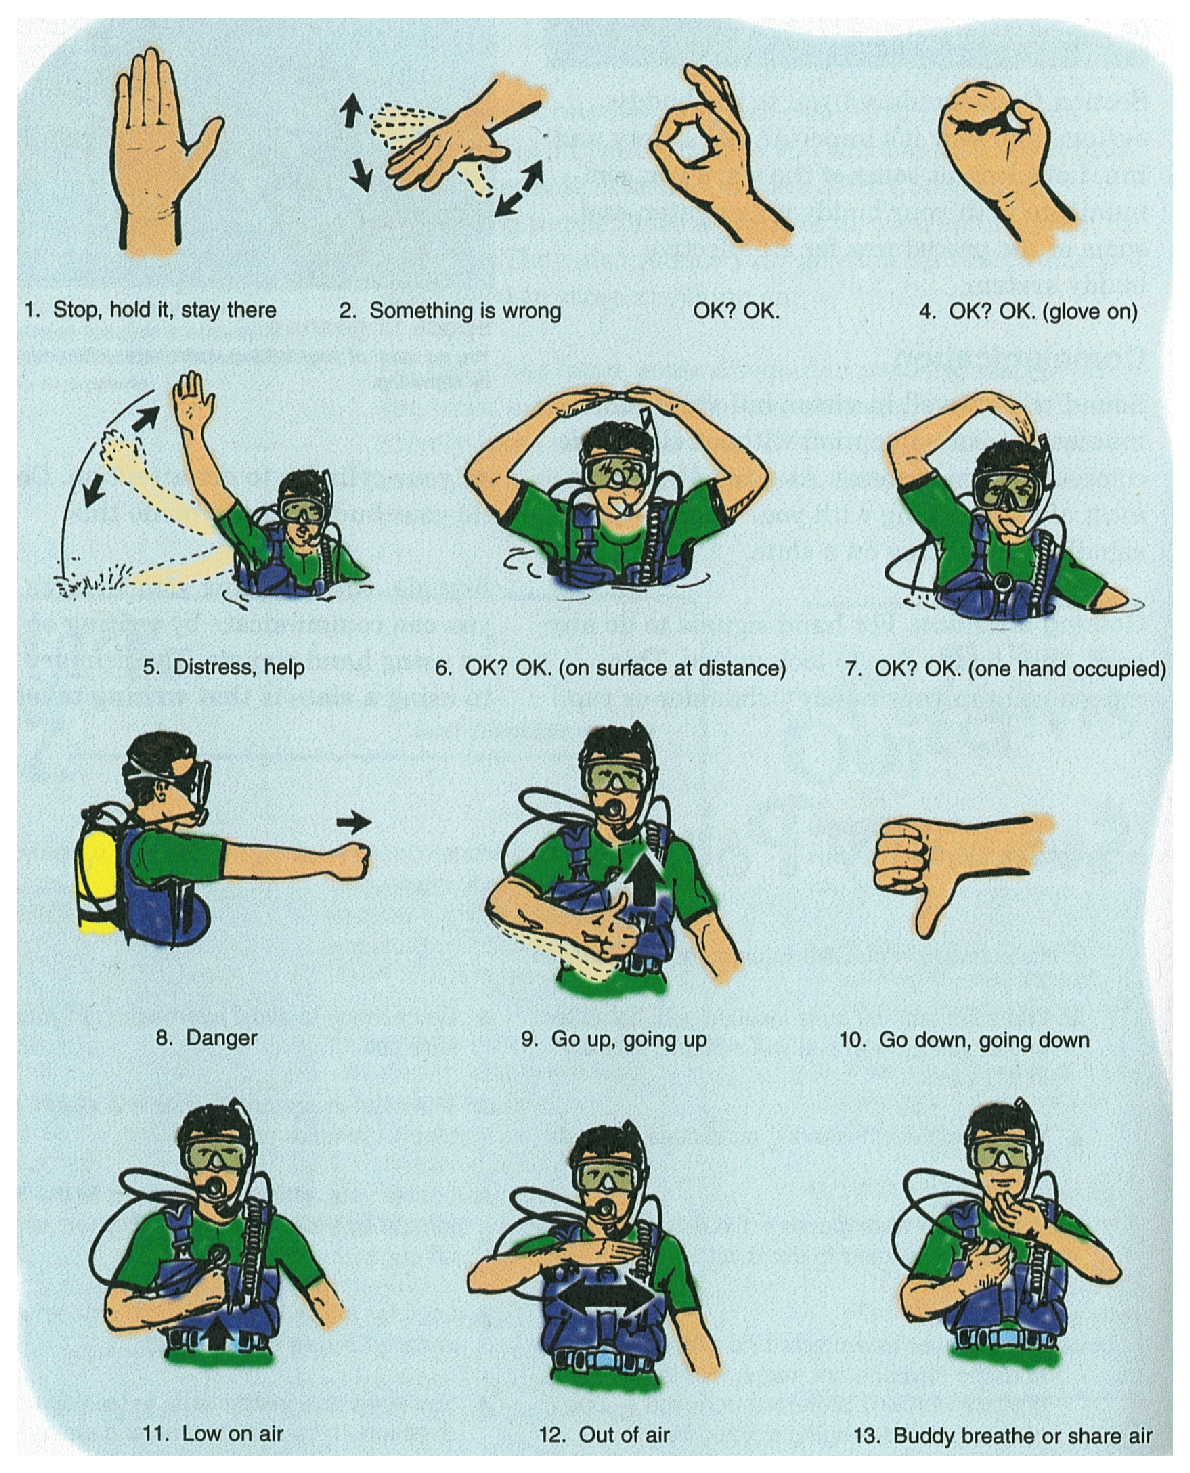
\includegraphics[width=3.22in]{hand-signals-1}
		\end{minipage}
		\hfill
		\begin{minipage}{0.48\textwidth}
			\raggedright 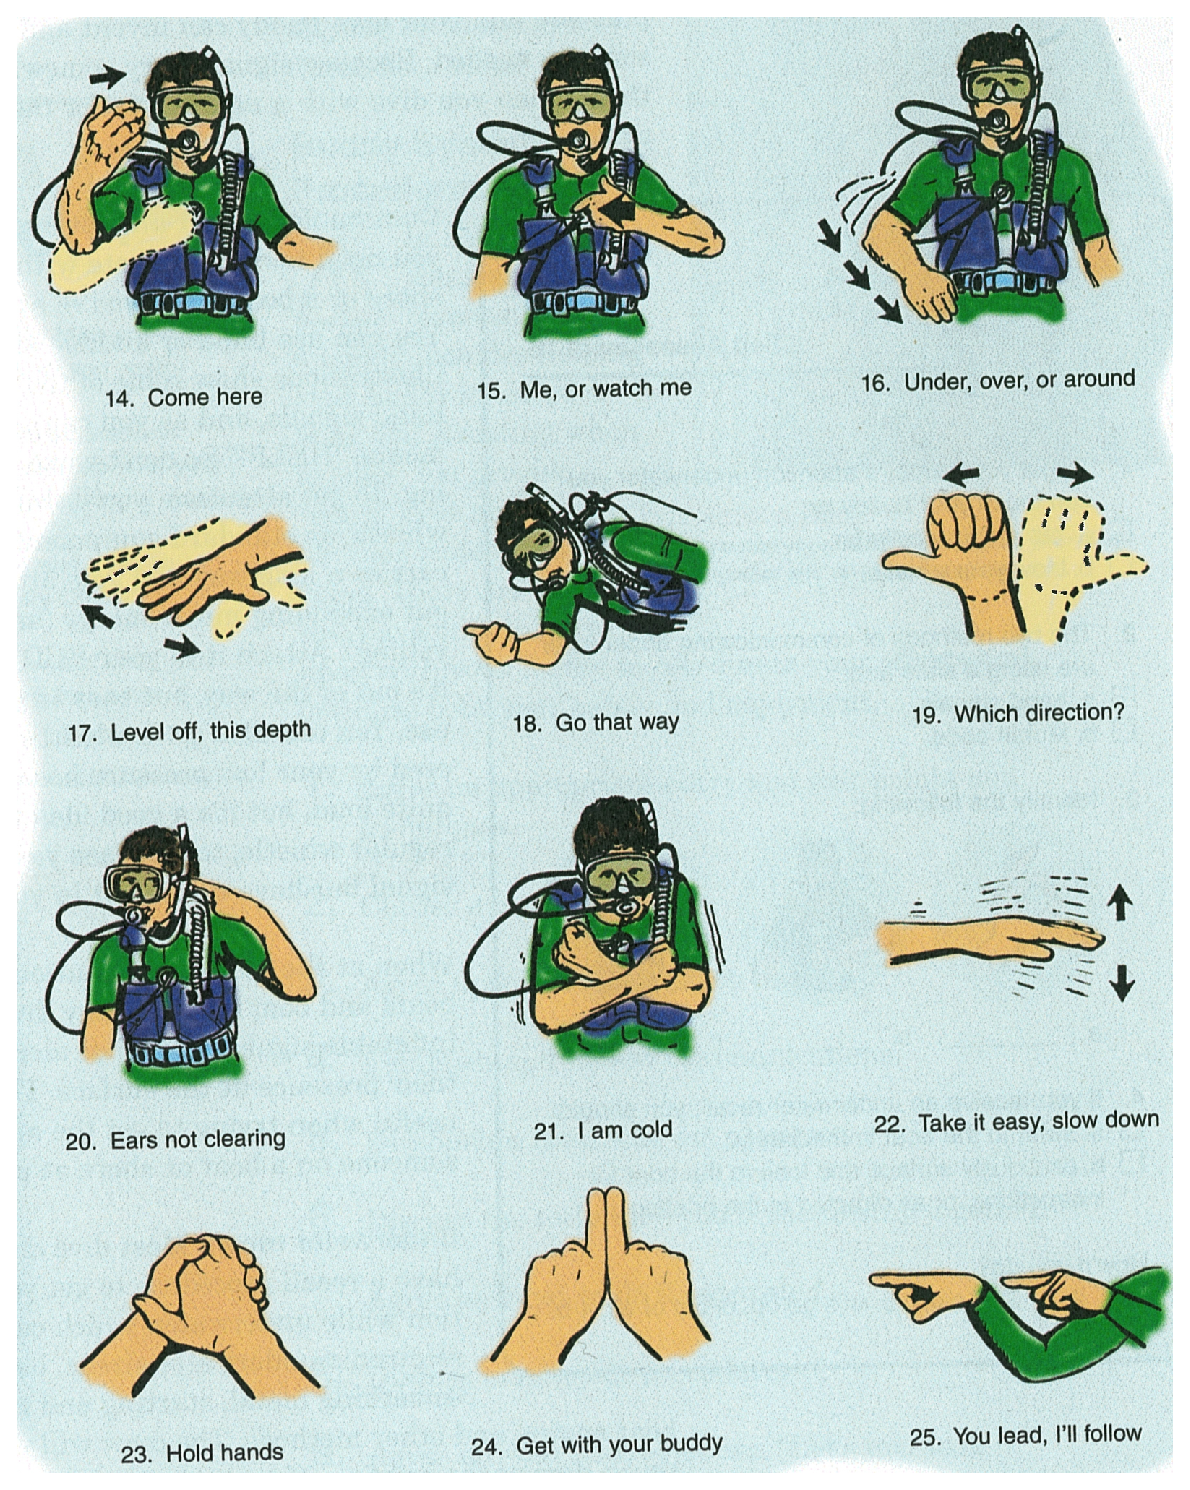
\includegraphics[width=3.22in]{hand-signals-2}
		\end{minipage}

		\caption{Hand signals.}
		\label{fig:handsignals}
	\end{figure}

	% 44.
	\begin{qanda}
		\begin{question}
What should you do if you get an underwater recall?
		\end{question}

		\begin{answer}
Cautiously surface and look to the boat for instructions.  Don't swim toward the boat until the captain signals that it's okay to do so.
		\end{answer}
	\end{qanda}

	% 45.
	\begin{qanda}
		\begin{question}
What nine considerations should you discuss with your buddy when planning a dive?
		\end{question}

		\begin{answer}
The nine considerations to discuss with your buddy when planning a dive are:
			\begin{nospacenumberedlist}
				\item Agree on appropriate entry and exit points and techniques
				\item Choose a course to follow
				\item Agree upon time and depth limits
				\item Establish and review communications
				\item Establish a returning air pressure
				\item Discuss the technique you'll use to stay together
				\item Agree on what to do if separated
				\item Discuss emergency procedures
				\item Agree on your dive objective
			\end{nospacenumberedlist}
		\end{answer}
	\end{qanda}

	% 46.
	\begin{qanda}
		\begin{question}
What are the steps of the Pre-dive Safety Check?
		\end{question}

		\begin{answer}
Use the phrase \textbf{Begin With Review And Friend} to help you remember the checks.
			\begin{nospacenumberedlist}
				\item \textbf{B} -- \textbf{B}CD -- Check adjustment, operation, low pressure inflator connection, and that the cylinder is firm in the band
				\item \textbf{W} -- \textbf{W}eights -- Check for proper weighting, and that the quick release system is clear for ditching.  Weight belts should have a right hand release
				\item \textbf{R} -- \textbf{R}eleases -- Make sure you're familiar with your buddy's releases and how they work.  Check each other to make sure they're secure
				\item \textbf{A} -- \textbf{A}ir -- Confirm that you both have ample air for the dive, that your valves are open, that regulators and alternate air sources work, and that you know where to find and how to use each other's alternate air sources
				\item \textbf{F} -- \textbf{F}inal Okay -- Give each other a final inspection looking for out of place equipment, dangling gauges, missing gear, etc
			\end{nospacenumberedlist}
		\end{answer}
	\end{qanda}

	% 47.
	\begin{qanda}
		\begin{question}
If you lose contact with your buddy underwater, what should you do?
		\end{question}

		\begin{answer}
Search for each other for not more than one minute, then surface and get back together.
		\end{answer}
	\end{qanda} 